\documentclass{standalone}
\usepackage{tikz}
\begin{document}
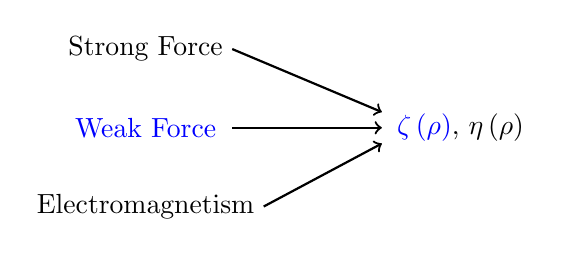
\begin{tikzpicture}
    \node[] at (-1, 1) {Strong Force};
    \node[] at (-1, 0) {\textcolor{blue}{Weak Force}};
    \node[] at (-1,-1) {Electromagnetism};
    \draw[thick, ->] (0.1, 1) -- (2, 0.2);
    \draw[thick, ->] (0.1, 0) -- (2, 0.0);
    \draw[thick, ->] (0.5,-1) -- (2,-0.2);
    \node[] at (3,0) {\textcolor{blue}{$\zeta\left(\rho\right)$}, $\eta\left(\rho\right)$};
\end{tikzpicture}
\end{document}

